\documentclass[final]{cvpr}

\usepackage{times}
\usepackage{epsfig}
\usepackage{graphicx}
\usepackage{amsmath}
\usepackage{amssymb}
\usepackage{tabularx}
\usepackage{siunitx}
\usepackage[pagebackref=true,breaklinks=true,colorlinks,bookmarks=false]{hyperref}

\graphicspath{{images/}}
\newcolumntype{Y}{>{\centering\arraybackslash}X}

\def\cvprPaperID{****} % *** Enter the CVPR Paper ID here
\def\confYear{CVPR 2021}
%\setcounter{page}{4321} % For final version only


\begin{document}
%%%%%%%%% TITLE
\title{DeepPhospho: A Transformer-based Deep Network for Peptide \\Tandem Mass Spectra Prediction}

\author{Weizhen Liu\textsuperscript{1}\thanks{Both authors contributed equally to the work.}, Rongjie Li\textsuperscript{1}\footnotemark[1], 
Ronghui Lou\textsuperscript{2,3,5}, 
Wenqing Shui\textsuperscript{2,3}\thanks{Both are conrresponding authors.}, 
Xuming He\textsuperscript{1,4}\footnotemark[2]\\
\textsuperscript{1}School of Information Science and Technology, ShanghaiTech University\\
\textsuperscript{2}School of Life Science and Technology, ShanghaiTech University\\
\textsuperscript{3}iHuman Institute, ShanghaiTech University\\
\textsuperscript{4}Shanghai Engineering Research Center of Intelligent Vision and Imaging\\
\textsuperscript{5}University of Chinese Academy of Sciences\\
{\tt\small \{liuwzh, lirj2, lourh, shuiwq, hexm\}@shanghaitech.edu.cn}
}

\maketitle

%%%%%%%%% ABSTRACT
\begin{abstract}
   In mass-spectrometry-based proteomics, the identification and quantification of peptides and proteins heavily
   rely on sequence database searching or spectral library matching. The size and quality of sequence database is
   crucial for the searching. There are researches that propose we could build a virtual sequence database composed
   of the peptide sequence with its retention time and spectra by computational method. Nowadays, the deep learning
   model has show its power in computer vision and natural language processing,
   however, in proteomics, the
   lack of accurate predictive models for
   fragment ion intensities and retention time impairs the realization of the full potential of these proposals.
   Here, we propose
   our new method DeepPhospho, based on LSTM-Transformer model, and focus on the phosphorylation peptide data, especially.
   Using our model, researchers could build a larger and more
   accurate peptide library for protein identification in mass-spectrometry-based proteomics.
\end{abstract}

%%%%%%%%% BODY TEXT

\section{Introduction}
%task description and challenges

A fundamental problem in proteome analysis is to seek a predictive relationship between a peptide and its measured chemico-physical properties, such as the chromatographic retention time (RT) and fragment ion intensity in LC-MS/MS~\cite{gessulat2019prosit}. In particular, bottom-up proteomic approaches can greatly benefit from
high-quality mass spectra prediction from amino acid sequences~\cite{gessulat2019prosit}.
However, such a prediction task is particularly challenging due to the complex quantum effect within peptides and noisy measurement process.

% what has done before

Recently, thanks to the availability of large-scale peptide databases, data-driven strategies have been adopted to tackle this problem~\cite{arnold2006machine}.
Notably, deep learning based approaches have shown promising performances in the task of retention time and/or mass spectrum estimation~\cite{zhou2017pdeep,ma2018improved,tiwary2019high,zeng2019ms,gessulat2019prosit}. The existing deep learning methods typically first embed amino acids into a vector representation, and then feed them into a multilayer neural network (CNN or LSTM) which extracts a global representation of the input peptide and predicts its retention time/ion intensity. Specifically, some of early works adopt convolutional neural networks (CNN) or its variants, which have limited capacity in modeling sequences of varying lengths and are largely restricted to predicting a single property of peptides (e.g., DeepRT~\cite{ma2018improved}). Recent efforts attempt to utilize recurrent neural networks, such as LSTMs~\cite{hochreiter1997long}, to capture the structural dependency in the peptide sequences~\cite{zeng2019ms}. Nevertheless, they only achieves limited success due to their restrictive structural assumption on the design of deep networks, including the linear embedding of amino acids and recurrent network topology.

% our idea and model design
%the long-range dependency
In this work, we present a novel deep learning framework, termed DeepPhospho, which tackles the challenge of peptide representation learning for RT and ion intensity prediction. To this end, we develop a hybrid deep network design, capable of better capturing the global structure of the peptide.
Specifically, we first employ a bi-LSTM network to compute the embedding of amino acids. This produces a context-aware local representations as each amino acid is enriched by the features of other amino acids in the same peptide. Given the new embedding, we then introduce a flexible Transformer-based network that uses self-attention to model long-range dependency in the peptide sequences. The Transformer module enables us to directly attend to multiple sites of the peptide, such as the pairs of b and y ion, without needing the recurrent computation. Finally, the network outputs a new representation for the input peptide, which is then fed into a linear regressor to generate predictions for RT or ion intensities.

We demonstrate the efficacy of the DeepPhospho on multiple challenging benchmarks of RT/ion-intensity prediction and provide detailed ablative study on the model design. Moreover, we have built a ready-to-use web server based on our model for the scientific community \footnote{\url{https://xxx.shanghaitech.edu.cn/xxx}}, and will also release our code(\url{https://github.com/weizhenFrank/DeepPhospho.git}).

%To the best of our knowledge, DeepPhospho is the first work to utilize the Transformer on the peptide spectrum prediction though it has been prevalently used in the natural language processing domain.

%In this work, we develop a novel deep learning framework, termed DeepPhospho, capable of better capturing the local and global property of the peptide, as well as its phosphine modification cues.
%by exploiting a large amount of peptide retention time and mass spectra data.
%In particular, our design takes into account the phosphine modification in model training/inference, which improves the prediction quality of ion intensity.


%We use the LSTM + Transformer as its architecture; the LSTM could learn a good amino acid representation for the downstream Transformer module. By exploiting self-attention, the Transformer module could capture the difference of amino acids much more precisely. More importantly, the self-attention mechanism could potentially force model to attend the pair of b ion and y ion as these two ions are broke down at the same time in mass spectrometer.
%In the supplementary, we show the superiority of LSTM + Transformer compared to solely Transformer or LSTM.
%Based on the observation that the Transformer module needs the good initial embedding of amino acid, we wonder that if whether or not a convolutional neural network (CNN) could replace the LSTM module to learn a good representation of amino acid, and the results show that the LSTM module is better than the CNN module configured before the Transformer.
%In further, we want to know a purely deep CNN whether if better than the LSTM + Transformer; however, results show a deep CNN could not generalize well compared with LSTM + Transformer architecture.



%There have been several tools that successfully utilized deep learning in RT and Ion intensity prediction, such as DeepRT\cite{ma2018improved} and pDeep2\cite{zeng2019ms}.

%DeepRT use the capsule network (CapsNet) \cite{sabour2017dynamic}  model to predict RT. However, the DeepRT did not explain very well for the choice of CapsNet, and CapsNet's structure cannot fully utilize the sequence's characteristics.

%pDeep2 just use the bi-directional LSTM model to predict the ion intensity, and it does not explicitly take the relations of amino acids into the consideration of model design.

% Our model design



\section{Related Work}
\subsection{Retention Time Prediction}
For retention time prediction, efforts to date to predict peptide RTs are mainly based on retention coefficients (Rc) of amino acids,
while SSRCalc~\cite{guo1986prediction} is the most popular Rc-based predictor. Rc is a parameter to appraise the contribution of an individual amino
acid to peptide RT, and the sum of all the Rcs of amino acids in a peptide could serve for RT estimation.
Additional factors such as peptide length, charge, and helicity are also considered during peptide RT prediction.
Several predictors based on Rc and other measurable factors have been proposed and reported in some studies. For example, Elude~\cite{moruz2010training,moruz2012chromatographic} and GPTime~\cite{maboudi2017uncertainty} developed from support vector machine (SVM) and Gaussian process
regression employed Rcs learned from data sets and can also provide RT prediction for post-translationally modified (PTM) peptides.
All these tools produced RT with $R^2$ values of less than 0.965 on various data sets. On the other hand, it is well recognized
that we are still lacking of enough knowledge to fully understand the physicochemical properties of peptides and the complex
interactions between peptides and stationary phase, which leads to the less-than optimum prediction of peptide RT. In terms
of the algorithm, the traditional model shows its limitation in tracing the many subtle factors that affect the peptide behaviors
on LC. Hence, in the field of peptide RT prediction, there is still large room for improvement.

Deep learning, an advanced machine learning method, has shown extraordinary capability to learn complex relationships
from large-scale data. There have been several tools that successfully utilized deep learning in RT prediction, such as
DeepRT~\cite{ma2018improved}, and Prosit~\cite{gessulat2019prosit}.

DeepRT use the capsule network (CapsNet)~\cite{sabour2017dynamic}
model. DeepRT could foresaw the RTs for the peptides at even different modification status included as oxidation of methionine, phosphorylation of
serine, threonine, tyrosine and at varied LC conditions included RPLC, SCX, HILIC.
Prosit utilizes the LTSM model and like the DeepRT, it could predict the retention time given the peptide sequence.
However, the DeepRT did not explain very well for the choice of CapsNet, and it did not fully consider the sequence's characteristics.
Prosit use the LSTM model to capture the this pattern. But, LSTM model has been beaten by the transformer model
in multiple tasks~\cite{vaswani2017attention}. Herein, we select the LSTM+transformer architecture.

\subsection{Ion Intensity Prediction}
Investigation of the peptide fragmentation is valuable both in theory and in practice. There are some researchers
focusing on the prediction of theoretical MS/MS spectra of peptides, including kinetic model-based methods and machine
learning based methods. MassAnalyzer~\cite{zhang2004prediction, zhang2005prediction} and MS-Simulator~\cite{sun2012ms,wang2015openms}
are two major kinetic model-based tools designed based on
the mobile proton hypothesis with some basic assumptions, and the key parameters of the models are tuned to fit the data
by statistics. The disadvantage of the kinetic model is that it cannot consistently be used to model the peptide
fragmentation under HCD, ETD, or electron-transfer and higher-energy collision dissociation (EThcD). PeptideART is
 a pure machine learning based tool which models the theoretical spectrum prediction as a classification problem, and
 the probability of the occurrence of each peak is learned by using a shallow feed-forward neural network~\cite{arnold2006machine,li2011accuracy}.
 Other previous work~\cite{frank2009ranking} predicts intensity ranks instead of relative intensities using learning-to-rank algorithms.
 It has been shown that a good prediction method can boost the identification of peptides. However, peptide
 fragmentation is very complex to predict; Li et al.~\cite{li2011accuracy} pointed out that the cross experiment correlations of PeptideART
 based on collision induced dissociation (CID) spectra were significantly lower than within-experiment analyses. To
 handle the complexity of peptide fragmentation, more powerful algorithms such as deep learning should be considered.

pDeep~\cite{zhou2017pdeep}, a deep learning-based method based on LSTM model to predict the intensity distribution of product ions of a peptide. pDeep can
work well in predicting not only HCD spectra but also ETD and EThcD spectra.pDeep achieved  $>$0.9 median PCCs (Pearson correlation coefficient)
in predicting HCD, ETD, and EThcD spectra, which is significantly higher than kinetic model-based MassAnalyzer and MS-Simulator as well
as the machine learning-based PeptideART. But, similarly like the RT prediction task, LSTM could not learn better than transformer, and this is why
we also choose the LSTM + transformer architecture for this task. After pDeep, the modified version of pDeep, called pDeep2~\cite{zeng2019ms}.

pDeep2 is spectrum predictor for modified peptides based on the deep learning model. It use the transfer-learning technique to transfer pDeep model
parameters to the prediction of modified peptide's spectrum. It claims that it's accurate model for predicting the spectra of peptides with common PTMs or low-abundance PTMs,
even if we only had a limited scale of benchmark modified PSMs.  Similarly, our model design make us to predict the spectrum of modified peptide.

\section{Methods}

It could be formulated as a regression problem from sequence to value: given sequence \( X \), a learned
function \( F \) could map the \( X \) to the \( y \), either retention time or ion intensity. The mathematical expression is as follows:
\[ \hat{y} = F(X;\Theta) \]
$\Theta$ is the parameters of the model.we find the optimal parameters \( \Theta^\star\) by minimizing  the loss function \( L \).
\[ \Theta^\star = \arg\min_{\Theta} L(\hat{y}, y) \]
We use the LSTM + Transformer model to solve the retention time (RT) and ion intensity prediction task.
The long short-term memory (LSTM)~\cite{hochreiter1997long} module comprises of two stacks of bi-directional LSTM. For each stack of LSTM, it has two layers and the dimension of input embedding and hidden state are 256 and 512, respectively. After one stack of LSTM, a combination of LeakyReLU-dropout-linear layer is configured. LSTM is a kind of recurrent neural network(RNN) trying to use gate function to capture the long dependency in the input sequence. The bi-directional LSTM, expecting to learn a good token embedding for the network's downstream layers, is scheduled as the first module of our model.

Transformer~\cite{vaswani2017attention} is the second module composed of n Transformer encoder.
Each Transformer encoder has 8 attention head, then a feedforward layer configured after attention head.


Transformer is an entirely different model by exploiting the self-attention compared to RNN.
Self-attention is an attention mechanism relating different positions of a single sequence to compute a representation of the sequence. Self-attention has been used successfully in a variety of tasks, including reading
comprehension, textual entailment, and learning task-independent sentence representations.
The Transformer is the first transduction model relying entirely on self-attention to compute its input and output representations without using sequence-aligned RNNs or convolution. It has achieved state-of-the-art performance in multiple natural language tasks, such as language translation, language entailment classification, language modeling, etc. We use the pre-layer form of Transformer, which is proposed in~\cite{xiong2020layer} and converges much faster.

The position encoding by sine and cosine functions is added to the output of LSTM module then feed into the Transformer module.
We take the same way of position encoding as~\cite{vaswani2017attention} which is as follows:
\begin{align*}
    PE_{(pos, 2i)} &= \sin{(pos/10000^{\frac{2i}{d_{model}}})} \\
    PE_{(pos, 2i+1)} &= \cos{(pos/10000^{\frac{2i}{d_{model}}})}
\end{align*}
where $pos$  is the position, $i$ is the dimension and $d_{model}$ have the same dimensions with input embeddings.


\subsection{RT prediction model}
For this task, we use model ensemble method and implement
5 models with two units of two layers bi-directional LSTM and 4, 5, 6, 7, 8 Transformer encoder layers, correspondingly. We train and select those 5 models independently. After obtaining the best models, those 5 predictions of retention time are averaged as the final prediction for each peptide.

The amino acid tokens are embedded into 256 dimensions to the neural network.
Especially since the output of the Transformer is the same length as the input sequence, we need to take it down to one scaler for retention time. By adding the time distributed linear layer to assign varied weights for different amino acids dynamically, we obtain RT prediction.


%-------------------------------------------------------------------------
\subsection{Ion intensity prediction model}

We implement one model for ion intensity prediction, which has two units of two layers bi-directional LSTM and 8 layers of Transformer encoder. Like the RT prediction task, we first embed the amino acids token, the charge to 192, 64 dimensions separately then concatenate those two vectors, forming the 256 dimension vectors to the neural network. The last layer is a linear layer, which projects the feature from high dimension to 8 dimensions with length unchanged as our prediction of ion intensity.



\subsection{Metric}
For the RT task, the $\Delta$$t_{95\%}$ metric is used as the primary metric, representing the minimal time window containing the deviations between observed and predicted RTs for 95\% of the peptides.
\[ \Delta t_{95\%} = 2 * | y - \hat{y} |_{95\%} \]
The subscript 95\% means the 95\% rank of the deviations.
Pearson Correlation Coefficient (PCC) is also referred to, but we select the model by $\Delta$$t_{95\%}$ metric as the PCC metric could not reflect the difference between different methods as could be seen in the following experimental results.

For the Ion Intensity task, We compute each peptide's PCC and select the median of those PCCs as the final evaluation metric. Primarily, we follow Prosit~\cite{gessulat2019prosit} using normalized
spectral angle(SA) as another metric, and the median of those SAs is reported.
SA's formula is as follows.
\[ SA = 1 - 2 * \frac{cos^{-1}(\hat{V_a}\cdot\hat{V_b})}{\pi} \]
$\hat{V}$ is a vector whose L2 norm equals 1. We select the model by the median PCC metric.

\section{Experiments}

\subsection{Dataset}
\paragraph*{Data composition and preprocess}
The sequence is represented by the symbol of amino acids such as L, K, M, etc., typically 7-50 in length. Specially, we use 1 to represent the oxidation of methionine (M), and we use 2,3,4 to represent the phosphorylation of serine(S), threonine(T), tyrosine(Y), respectively. In further, we support the peptide with N-terminal acetyl modification. We use the * symbol to indicate modification, @ to indicate no modification. 

% Retention time (RT) is a measure of the time taken for a solute to pass through a chromatography column.
% It is calculated as the time from injection to detection.
For RT datasets, they are comprised of \( \{X, y\} \) pair. 
$X:= \{ <x_0, x_1, x_2, x_3,\dots, x_i, \dots, x_n>\}$. $x_0$ is the symbol of * or @. 
$x_i$ ($i>= 1$) is amino acid. $n$ is the length of peptide. \( y \) is the retention time. 
As the retention time is distributed in the real-world unit, such as minutes or seconds, we scale each dataset by its maximal and minimal of retention time to 0 - 1 by the following formula. 
\[RT_{normalized} =  \frac{RT-min(RT)}{max(RT)-min(RT)}\]

To train a better model, we sequentially pre-train the models in four datasets called 
HumanPhosDB~\cite{lawrence2016plug}, Jeff~\cite{liu2018vivo}, VeroE6~\cite{bouhaddou2020global}
and R2P2~\cite{leutert2019r2}. We split those pre-training datasets into training and validation set, selecting the best model on the validation set. The model is initialized by the selected model before training on the next pre-training dataset until those four datasets are all trained on. There are three downstream datasets called U2OS-DIA~\cite{wang2020naguider},
RPE1-DIA~\cite{bekker2020rapid} and RPE1-DDA~\cite{bekker2020rapid}. For the three downstream datasets, we manually set the $min(RT)$ and $max(RT)$ equals -100 and 200, respectively. -100 and 200 cold cover all the RTs in the three datasets and the following researcher could directly use our well trained model and the fixed $min(RT)$ and $max(RT)$ to predict the unknown RTs of their interested peptides.

Ion intensity datasets are also comprised of \( \{X, y\} \) pair. 
$X := \{ <x_0, x_1, x_2, x_3,\dots, x_i, \dots, x_n, +q> \}$. $+q$
is the charge carried by the peptide sequence before it is fragmented in the mass spectrometer. \( y \) is the spectrum of the peptide. Each y is composed of pairs of key and value.
The key is the ion's name, such as y2+1, b6+2, and the value is their corresponding raw intensity.
We divide each intensity by the maximum of the intensities within a peptide sequence to normalize each intensity into 0-1. As kinds of ions in the dataset is severely imbalanced, we only select the 8 types of ions same as pdeep2, that is b(y)i+1-noloss, b(y)i+2-noloss, b(y)i+1-1,H3PO4 and b(y)i+2-1,H3PO4, i indicating the site of b(y)ion to train and predict. The shape of ion intensity input is illustrated in the supplementary.

Similarly to the RT task, we also use those ion intensity in three of four pre-training dataset Jeff~\cite{liu2018vivo}, VeroE6~\cite{bouhaddou2020global} and R2P2~\cite{leutert2019r2}, and fine-tune the pre-trained model on the downstream dataset U2OS-DIA~\cite{wang2020naguider}, RPE1-DIA~\cite{bekker2020rapid} and RPE1-DDA~\cite{bekker2020rapid}. The summary of the datasets used in this work is shown in Table~\ref{table:Datasets}.
\paragraph*{Metric} For RT task, the $\Delta$$t_{95\%}$ metric is used as the main metric, which represents the minimal time window containing the deviations between observed and predicted RTs for 95\% of the peptides.
\[ \Delta t_{95\%} = 2 * | y - \hat{y} |_{95\%} \]
The subscript 95\% means the 95\% rank of the deviations.
We select the model by $\Delta$$t_{95\%}$ metric.
Pearson Correlation Coefficient (PCC) is also referred.

For Ion Intensity task, We compute each peptide's PCC and select the median of those PCCs as the final evaluation metric.
Primarily, we follow Prosit~\cite{gessulat2019prosit} using normalized
spectral angle(SA) as another metric and the median of those SAs is reported.
SA's formula is as follows.
\[ SA = 1 - 2 * \frac{cos^{-1}(\hat{V_a}\cdot\hat{V_b})}{\pi} \]
$\hat{V}$ is a vector whose L2 norm equals 1. We select the model by the median PCC metric.

\subsection{RT experiments}
We sequentially train the model on the four pre-training datasets, and obtain the best model by the validation sets. Then we fine-tune the model on the three downstream datasets, respectively. 
The downstream datasets are split into training : validation : test = 8 : 1 : 1, and we select model on the validation set, reporting the metric on the test set.  
Correspondingly, we download the DeepRT model provided by the \cite{ma2018improved}, and fine tune the model on those downstream datasets. The detailed results is shown in Table 

\subsection{Ion Intensity experiments}
As we have explore the architecture in the RT task, so that we only compare with the pdeep2.
The DDA comparison is shown in Figure \ref{fig:DDA}, Table \ref{table:DDA} and Figure \ref{fig:DIA18},
Table \ref{table:DIA18}.
From the results, we could see that in the metric median PCC and SA, we have beaten the SOTA model
pdeep2. In further, to explain our model's good generalization ability, we train our model in the DDA
dataset and direct test on the DIA18 dataset. Results are show in the Figure \ref{fig:DIA18_direct} and Table \ref{table:DIA18_direct}.
And we could see results that model trained on the DDA dataset, test on DIA18 dataset are comparable to trained
on DIA18, and are even similar to pdeep2's results on DIA18.
%-------------------------------------------------------------------------

\subsection{ablation study}

%\begin{figure}[t]
%
%   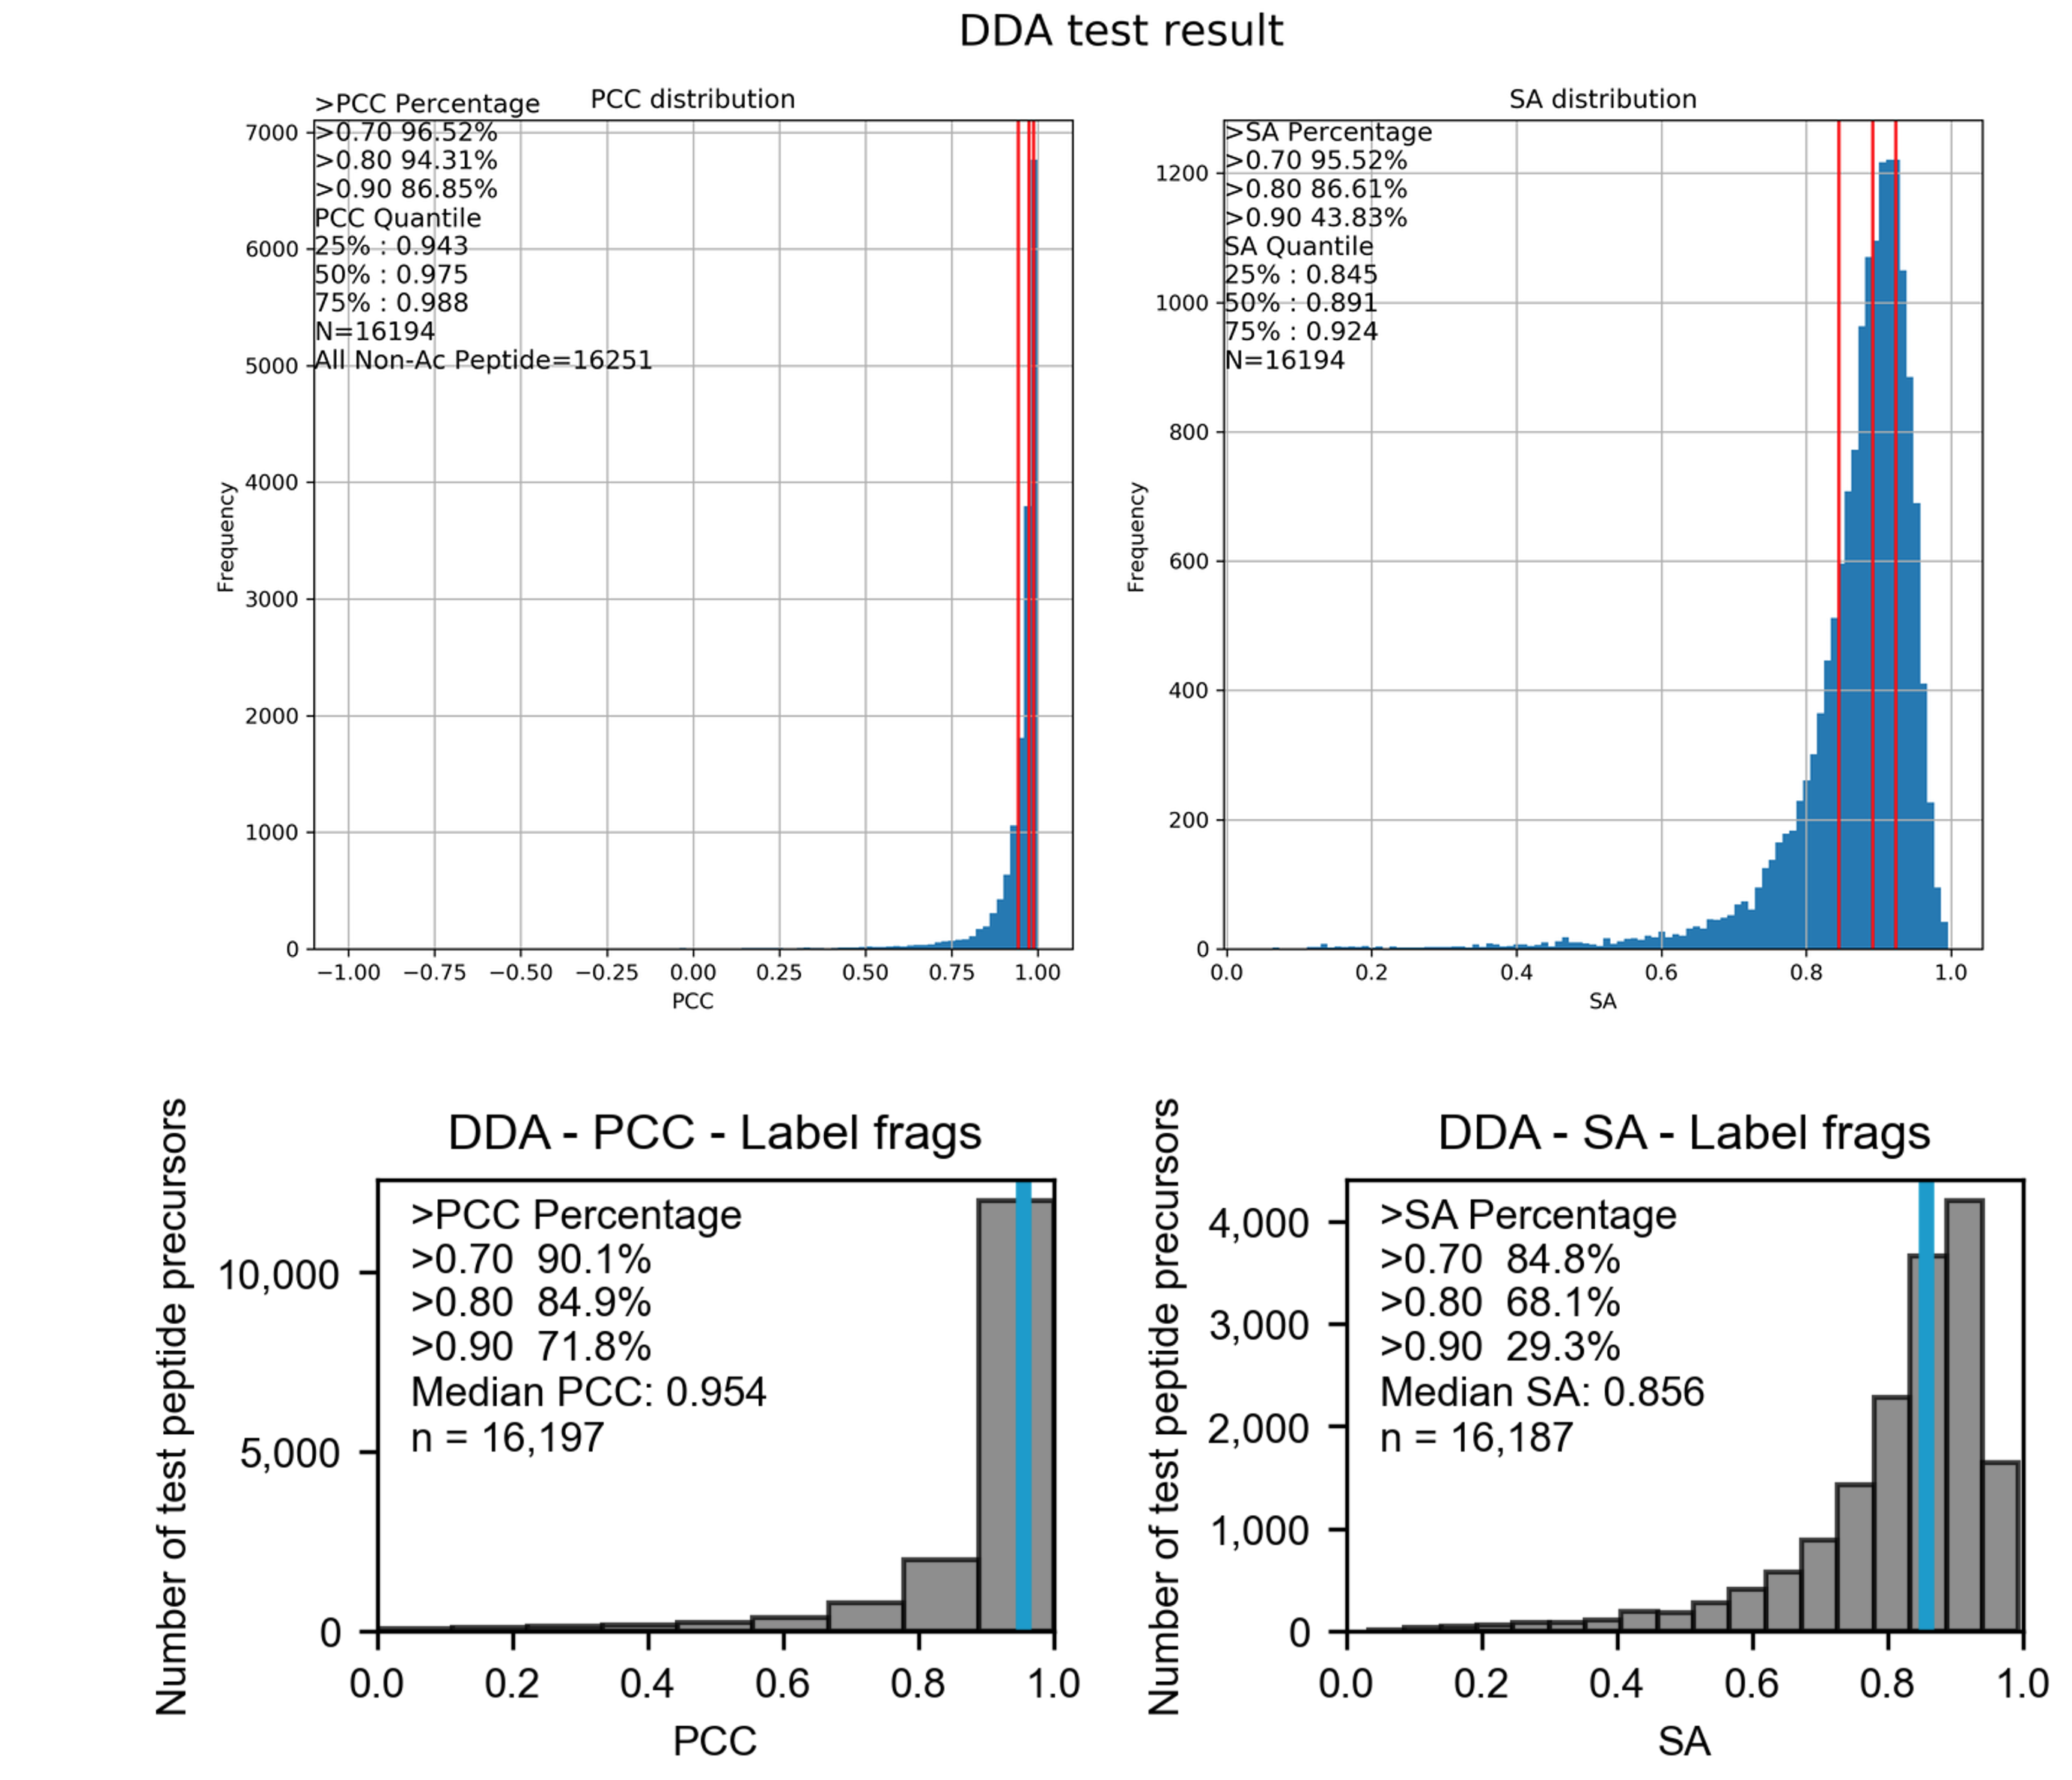
\includegraphics[width=3.0in]{DDA}
%
%   \caption{Visualization of performance of DDA dataset. The above is ours and the below is pdeep2}
%\label{fig:DDA}
%\end{figure}
%
%
%\begin{figure}[t]
%
%   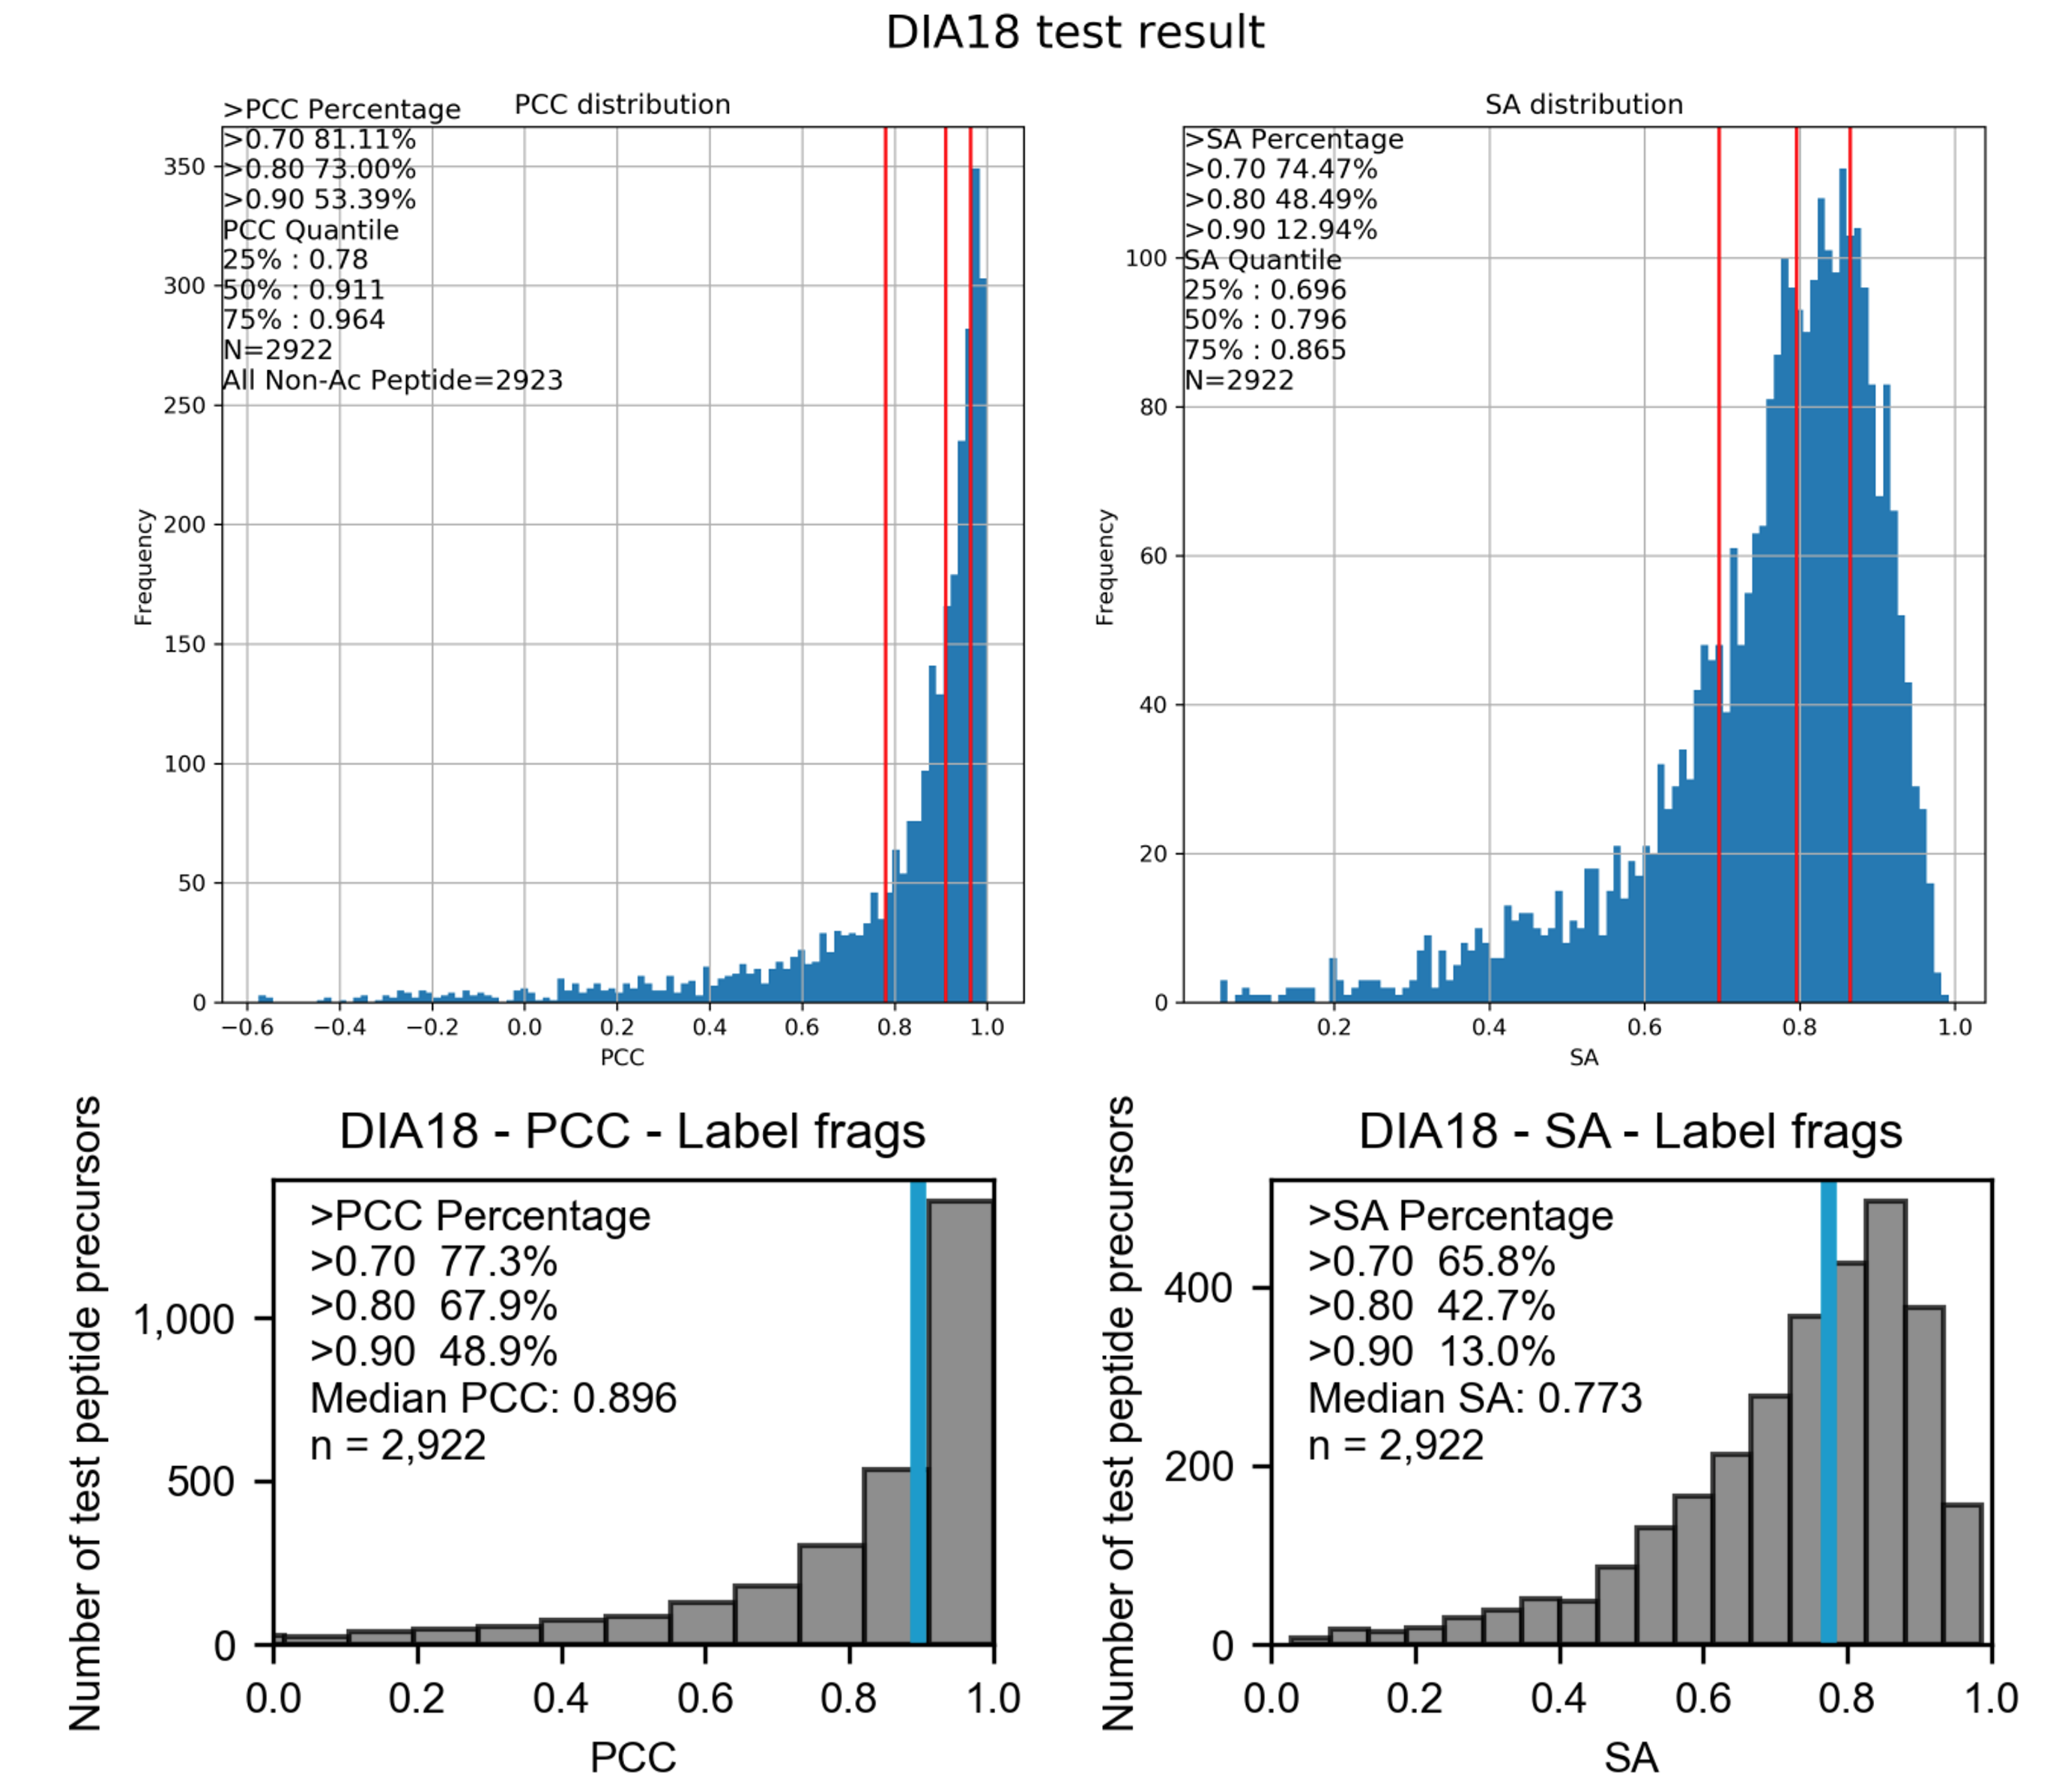
\includegraphics[width=3.0in]{DIA18}
%
%   \caption{Visualization of DIA18 dataset. The above is ours and the below is pdeep2}
%\label{fig:DIA18}
%\end{figure}
%
%
%\begin{figure}[t]
%
%   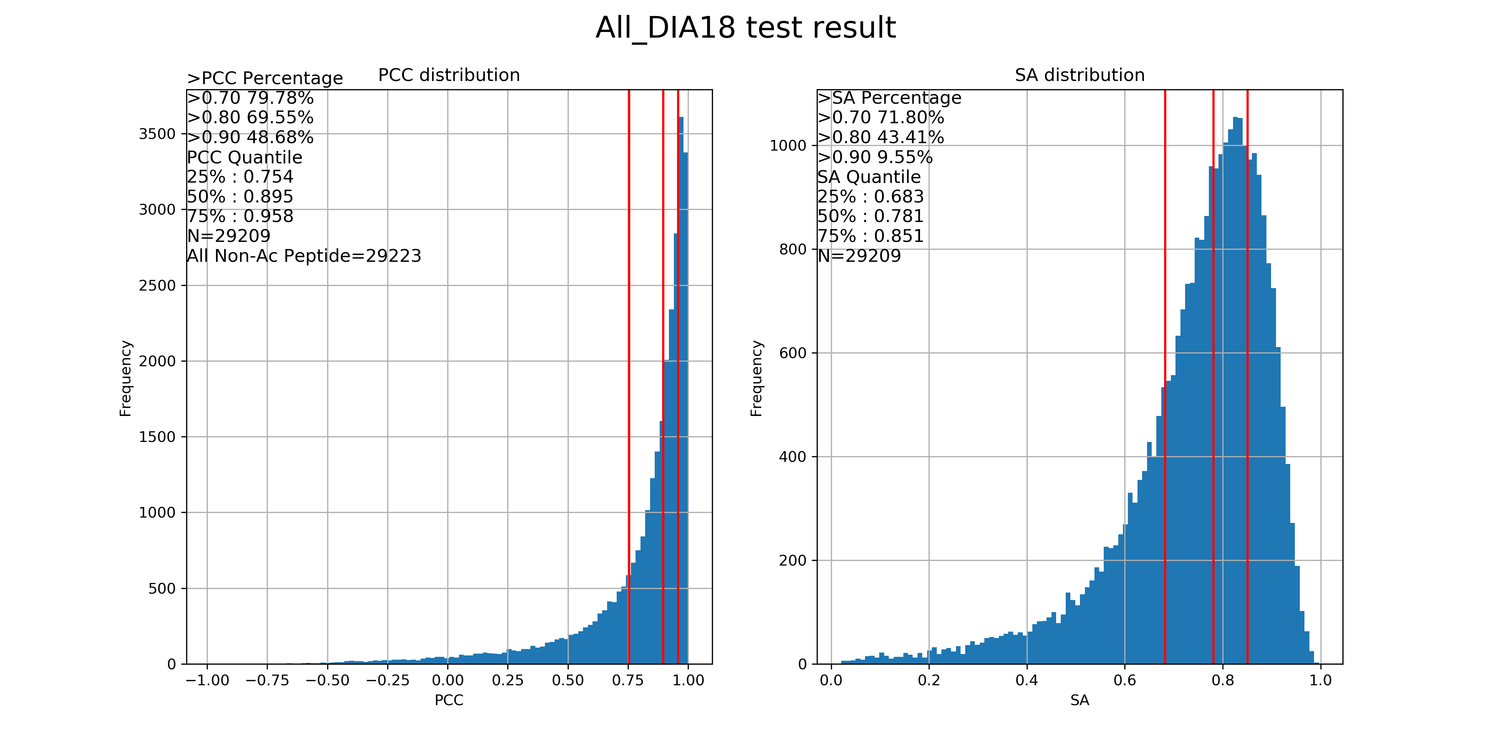
\includegraphics[width=3.5in]{DIA_direct_test}
%
%   \caption{Direct test on DIA18 dataset.}
%\label{fig:DIA18_direct}
%\end{figure}
%

\begin{table}
    \begin{center}
    \begin{tabularx}{\columnwidth}{|m{0.3\columnwidth}|Y|Y|}
    \hline
    data description & no. of peptides & no. of spectra\\
    \hline
    HumanPhosDB~\cite{lawrence2016plug} & 204,558 & -\\
    Jeff~\cite{liu2018vivo} & 67,552 & 89,437\\
    VeroE6~\cite{bouhaddou2020global} & 43,405  & 54,004\\
    R2P2~\cite{leutert2019r2} & 35,808 & 43,312\\
    U2OS-DIA~\cite{wang2020naguider} & 48,327 & 58,843\\
    RPE1-DIA~\cite{bekker2020rapid} & 33,576 & 39,977\\
    RPE1-DDA~\cite{bekker2020rapid} & 129,109 & 165,719\\
    \hline
    \end{tabularx}
    \end{center}
    \caption{Retention time datasets}
    \label{table:Datasets}
    \end{table}
 
    \begin{table}
       \begin{center}
      \resizebox{\columnwidth}{!}$ where the lower is the better, and the right is PCC where the higher is the better.}
       \label{table:Jeff}
       \end{table}
 
 \begin{table}
    \begin{center}
    \begin{tabular}{|l|c|c|}
    \hline
    Model & Median PCC & Median SA \\
    \hline\hline
    pdeep2 & 0.954 & 0.856 \\
    DeepPhospho$\star$ & 0.975 & 0.891 \\
    \hline
    \end{tabular}
    \end{center}
    \caption{DDA Dataset results.Ours is better.}
    \label{table:DDA}
    \end{table}
 
 \begin{table}
    \begin{center}
    \begin{tabular}{|l|c|c|}
    \hline
    Model & Median PCC & Median SA \\
    \hline\hline
    pdeep2 & 0.896 & 0.773 \\
    DeepPhospho$\star$ & 0.911 & 0.796 \\
    \hline
    \end{tabular}
    \end{center}
    \caption{DIA18 Dataset results.Ours is better.}
    \label{table:DIA18}
 \end{table}
 
 \begin{table}
    \begin{center}
    \begin{tabular}{|l|c|c|}
    \hline
    Model & Median PCC & Median SA \\
    \hline\hline
    Direct Test & 0.895 & 0.781 \\
    Train then Test & 0.911 & 0.796 \\
    \hline
    \end{tabular}
    \end{center}
    \caption{DIA18 Dataset results. Direct test only drops little compared to training and test}
    \label{table:DIA18_direct}
 \end{table}
 %%-------------------------------------------------------------------------

\section{Conclusion}
In this study, we introduce DeepPhospho, a flexible deep neural network based on the LSTM-Transformer architecture able to predict retention times and tandem mass spectrometry spectra of peptides and it substantially surpasses current methods in several datasets. We design our method target on the phosphorylated peptides.

Our collaborator's results demonstrate that predicted spectral libraries can be used for analyzing DIA data. While predicted
libraries performed slightly worse than high-quality experimental spectral libraries, replacing lower quality
spectral libraries by consistent and high signal-to-noise predicted spectra increased the number of identified
peptides by up to 10$\%$. In the future, DeepPhospho might enable the regeneration of libraries on instrument replacement
or calibration and potentially supports the consistent addition of new peptide hypothesis without compromising
the homogeneity of a library.

{\small
\bibliographystyle{ieee_fullname}
\bibliography{egbib}
}

\end{document}
